\chapter{lmer output}
\footnote{Signif. codes:   ‘***’ 0.001 ‘**’ 0.01 ‘*’ 0.05 }
\begin{table}[htbp]
\caption{duration \& syllable quantity}
\begin{center}
\begin{tabular}{|l|c|c|c|}
\hline
{\bf Predictors}	&	{\bf Estimates}	&	{\bf Confidence Interval}	&	{\bf p}	\\
\hline
\hline
(Intercept)	&	0.27	&	0.23 – 0.30	&	<0.001***	\\
Q2	&	-0.04	&	-0.06 – -0.02	&	<0.001***	\\
Q3	&	-0.03	&	-0.06 – -0.00	&	0.048*	\\
off-ictus &	-0.05	&	-0.08 – -0.02	&	0.004*	\\
Q2 * off-ictus	&	0.02	&	-0.03 – 0.06	&	0.54	\\

Q3 *off-ictus	&	-0.02	&	-0.07 – 0.03	&	0.44	\\
\hline
\hline
$\sigma^2$ 	&	0.0012	&		&		\\
$\tau_{00}$ word	&	0.0034	&		&		\\
$\tau_{00}$ song	&	0.0022	&		&		\\
$\tau_{00}$ performer	&	0.0001	&		&		\\
ICC	&	0.8227	&		&		\\
\hline
\hline
N song	&	9	&		&		\\
N word	&	298	&		&		\\
N performer	&	3	&		&		\\
Observations	&	367	&		&		\\
Marginal R2 / Conditional R2	&	0.071 / 0.835	&		&		\\
\hline
\end{tabular}
\end{center}
\label{qdurrandoms}
\end{table}%



%%%%%%%%%%


\begin{table}[htb]
\caption{duration \& syllable quantity: model comparison (max to null)}
\centering
\begin{tabular}{|ccccccccc|}
\hline
      & npar   &  AIC   &  BIC & logLik & deviance  & Chisq & Df & Pr(>Chisq)    \\
      \hline
      \hline
null  &  5 &-914.74 &-895.21 &462.37  &-924.74        &&& \\                 
design  &  10 &-949.20 &-910.15 &484.60 & -969.20 & 44.464  &5  &1.865e-08 *** \\
\hline

\end{tabular}
\label{qcomp}
\end{table}%
%%%%%%%


\begin{table}[htb]
\caption{duration \& stress and ictus: model comparison (max to null) }
\begin{center}
\centering
\begin{tabular}{|ccccccccc|}
\hline
      & npar   &  AIC   &  BIC & logLik & deviance  & Chisq & Df & Pr(>Chisq)    \\
\hline
\hline
null &   5& -1747.0 &-1724.4  &878.5 & -1757.0         && \\            
design &   10& -1966.8& -1921.6  &993.4  &-1986.8 & 229.81&  5 & < 2.2e-16 ***\\
\hline

\end{tabular}
\end{center}
\label{durstrickmdls}
\end{table}%

%
%\begin{equation*}
%
%des_null_md: euclid ~ (1 | segment) + (1 | song) + (1 | performer) \\
%desmd: euclid ~ stressed + ictus + stressed * ictus + (1 | segment) + (1 | song) + (1 | performer) \\
%\end{equation*}





\begin{table}[htb]
\caption{duration \& stress-ictus}
\begin{center}
\begin{tabular}{|l|c|c|c|}
\hline
\hline
Predictors	&	Estimates	&	Confidence Intervals	&	p	\\
\hline
(Intercept)	&	0.22	&	0.18 – 0.25	&	<0.001***	\\
off-ictus	&	-0.03	&	-0.05 – -0.00	&	0.017**	\\
stressed	&	0.05	&	0.03 – 0.07	&	<0.001***	\\
Q2&	-0.05	&	-0.06 – -0.04	&	<0.001***	\\
off-ictus* stressed	&	-0.01	&	-0.04 – 0.02	&	0.467	\\
off-ictus* Q2	&	0.01	&	-0.01 – 0.03	&	0.332	\\
\hline
\hline
$\sigma^2$ 	&	0.0026	&&	\\
$\tau_{00}$ word	&	0.0004	&&	\\
$\tau_{00}$ song	&	0.0018		&&	\\
$\tau_{00}$ performer	&	0.0001		&&\\
ICC	&	0.4761	&&	\\
\hline
\hline
N word	&	315		&&	\\
N song	&	9		&&	\\
N performer	&	3	&&	\\
Observations	&	676	&&	\\
Marginal R2 / Conditional R2	&	0.190 / 0.576	&&\\
\hline
\end{tabular}
\end{center}
\label{durlmerrando}
\end{table}%

%%%space
%%%%%%%%%%%

\begin{table}[htb]
\caption{euclidean distance dependent fixed effects}
\begin{center}
\begin{tabular}{|l|c|c|c|}
\hline							
Predictors	&	Estimates	&	Confidence Interval	&	p	\\
\hline
\hline
(Intercept)	&	351.9	&	207.53 – 496.26	&	<0.001***	\\
stressed 	&	48.7	&	-48.46 – 145.87	&	0.325	\\
off-ictus	&	80.8	&	-14.93 – 176.52	&	0.098	\\
stressed*off-ictus	&		&		&		\\
\hline							
\hline
$\sigma^2$	&	32259.12			&&		\\
$\tau_{00}$ segment	&	4058.78		&&			\\
$\tau_{00}$  song	&	5512.35				&&	\\
$\tau_{00}$  performer	&	5432.4				&&	\\
ICC	&	0.32		&&			\\
\hline
\hline
N segment	&	11		&&			\\
N song	&	9				&&	\\
N performer	&	3		&&			\\
Observations	&	401				&&	\\
Marginal R2 / Conditional R2	&	0.008 / 0.323		&&			\\									
\hline							
\end{tabular}
\end{center}
\label{randolmereuc}
\end{table}%


\begin{table}[htb]
\caption{euclidean distance \& stress-ictus: model comparison (max to null) }
\begin{center}
\centering
\begin{tabular}{|ccccccccc|}

\hline
     &       npar  &  AIC   & BIC  & logLik & deviance  & Chisq & Df & Pr(>Chisq) \\
     \hline
     \hline
null  &  5 & 5347.3 & 5367.3 & -2668.7  & 5337.3             \\        
design    &      8 & 5348.7& 5380.7 &-2666.4  & 5332.7 & 4.5855 & 3   &  0.2048 \\
\hline
\end{tabular}
\end{center}
\label{aoveuc}
\end{table}%


%\begin{figure}[htb]
%\centering
%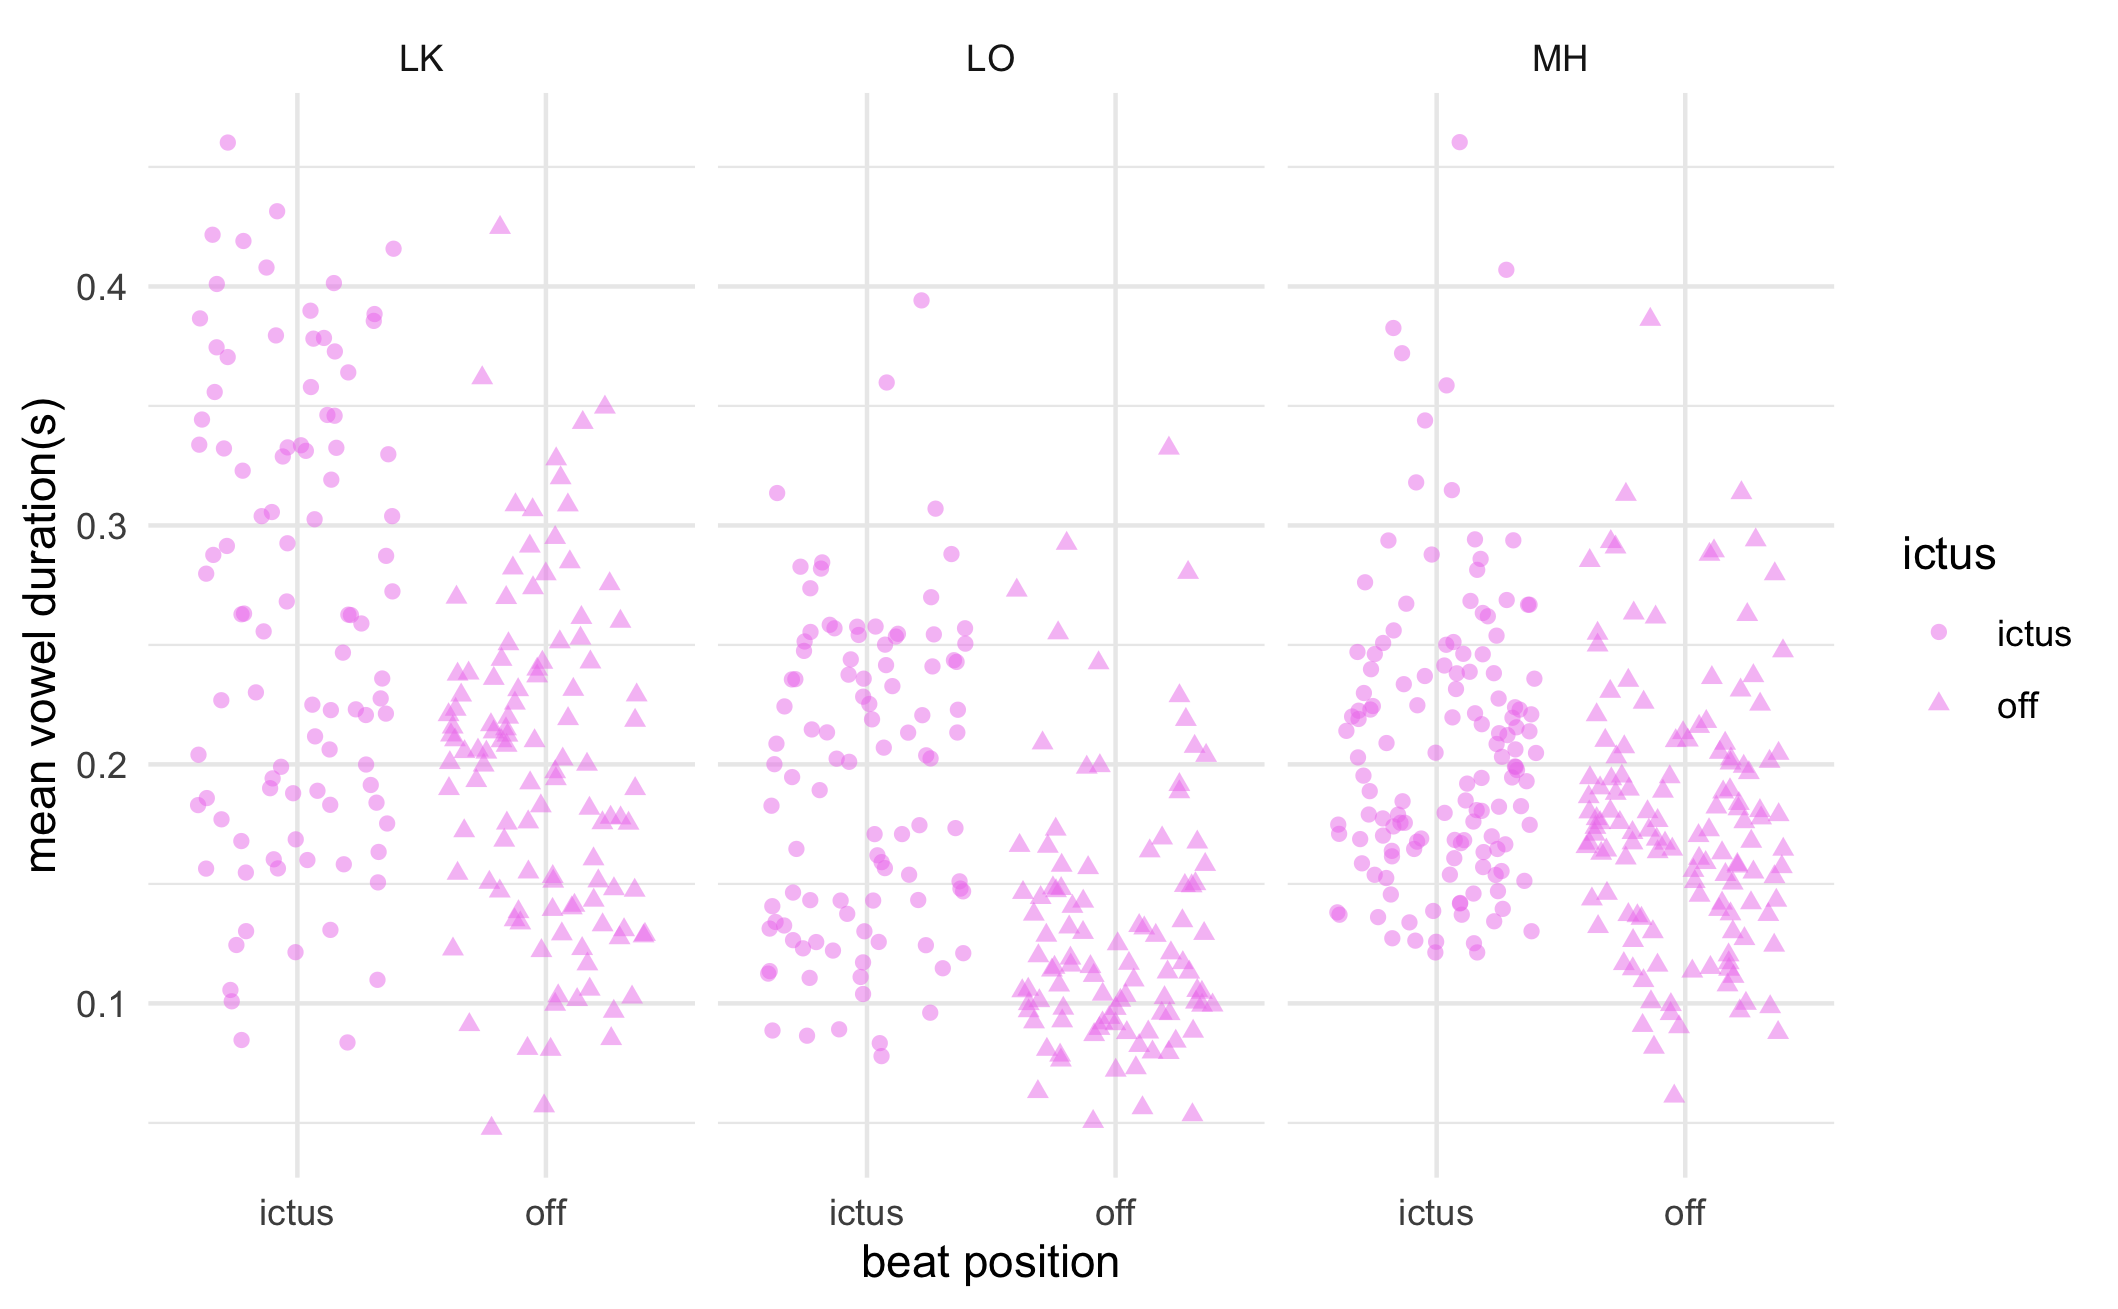
\includegraphics[width=\textwidth]{/Users/sarah/Git/regilaul_project/manuscript/results/perf_ick_dur.png}
%
%\caption{vowel durations on and off the beat in each performer}
%\label{perfbeats}
%
%
%\end{figure}

